\documentclass[aspectratio=169]{beamer}
\mode<presentation> {
\usetheme{default}
\usecolortheme{dolphin}
}
\usepackage{algorithm,algorithmic}
\usepackage{caption}
\usepackage{multirow}
\usepackage{threeparttable}
\usepackage{graphicx}
\usepackage{parskip}
\usepackage{float}
\usepackage{alphabeta}
\usepackage{multirow,array}
\usepackage{subfig}
\usepackage{amsmath}
\usepackage{amssymb}
\usepackage{mathabx}
\usepackage{caption}
\usepackage{pifont} 
\usepackage{booktabs,tabularx}
\usepackage{tikz}
\usetikzlibrary{shapes,arrows}
\usepackage[table]{xcolor}
\newcolumntype{Y}{>{\raggedright\arraybackslash}X}

\usepackage{tikz}
\usetikzlibrary{arrows.meta,positioning,calc,fit,backgrounds,decorations.pathreplacing, shapes.geometric}
\graphicspath{{figures/}}
\usetikzlibrary{matrix,chains,positioning,decorations.pathreplacing,arrows}

% TikZ Styles - Adjusted font sizes for clarity since bold is removed
\tikzset{
  >=Stealth,
  st/.style={circle,draw,inner sep=0pt,minimum size=6mm, fill=white}, 
  action/.style={circle,fill=black,inner sep=0pt,minimum size=2mm},
  tr/.style={-Stealth, line width=0.8pt},
  lbl/.style={font=\footnotesize},
  block/.style={rectangle, draw, fill=blue!10, rounded corners, minimum height=2em}
}

\newcommand{\E}{\mathbb{E}}
\newcommand{\R}{\mathbb{R}}
\newcommand{\1}{\mathbf{1}}
\newcommand{\loss}{\mathcal{L}}
\newcommand{\X}{\mathcal{X}}
\newcommand{\Y}{\mathcal{Y}}
\newcommand{\D}{\mathcal{D}}
\newcommand{\thetavec}{\boldsymbol{\theta}}
\DeclareMathOperator*{\argmax}{arg\,max}
\DeclareMathOperator*{\argmin}{arg\,min}
\setbeamertemplate{caption}[numbered]
\setbeamertemplate{navigation symbols}{}
\setbeamertemplate{footline}[frame number]

\title{Lecture 11: Unsupervised Learning}

\author{Yasuyuki Sawada, Yaolang Zhong}
\institute{University of Tokyo\\
  \small \texttt{\href{mailto:yaolang.zhong@e.u-tokyo.ac.jp}{yaolang.zhong@e.u-tokyo.ac.jp}}}
\date{\today}

\begin{document}

\begin{frame}
\titlepage  
\end{frame}

% Slide 2: Lecture Overview
\begin{frame}{Lecture Overview}
    \begin{enumerate}
        \item Recap: Classification
        \begin{itemize}
            \item Logistic Regression
            \item K-Nearest Neighbors (KNN)
        \end{itemize}
        \item Unsupervised Learning
        \begin{itemize}
            \item Task 1: Clustering (K-Means)
            \item Task 2: Dimensionality Reduction (PCA)
            \item Task 3: Density Estimation (KDE)
        \end{itemize}
    \end{enumerate}
\end{frame}


% Slide: Classification Recap
\begin{frame}{Recap: Classification and Logistic Regression}
    \small
    \begin{itemize}
        \item Setup: The response variable $Y$ is categorical, taking values in $\mathcal{C} = \{1,2,\dots,K\}$.
        \item Goal: Estimate conditional class probabilities $\hat{p}_c(x) = \Pr(Y = c \mid X = x)$, and assign observations to the class with highest probability.
        \item Loss Function: Misclassification rate $\frac{1}{n} \sum_{i=1}^n \1(y_i \neq \hat{y}_i)$.
        \item Example (Logistic Regression): For binary classification ($Y \in \{0,1\}$),
        \[
            \Pr(Y=1 \mid X) = \frac{e^{\beta_0 + \beta_1 X}}{1 + e^{\beta_0 + \beta_1 X}},
        \]
        where $\beta$ is estimated by maximum likelihood.
    \end{itemize}
\end{frame}

% Slide: KNN — Unified Introduction
\begin{frame}{K - Nearest Neighbors (KNN)}
    \small
    \begin{itemize}
        \item Alternative Approach: Instead of a global parametric model for $\Pr(Y \mid X)$, KNN constructs a local, data-driven approximation.
        \item Local Similarity Principle:
        \begin{itemize}
            \item For query point $x_0$, observations with covariates $x_i$ close to $x_0$ are most informative.
            \item Closeness is measured by a distance metric $d(x_i, x_0)$.
        \end{itemize}
        \item Local Probability Estimation: Let $\mathcal{N}_k(x_0)$ be the $k$ nearest neighbors of $x_0$.
        \[
            \hat{p}_c(x_0) = \frac{1}{k} \sum_{i \in \mathcal{N}_k(x_0)} \1(y_i = c).
        \]
        \item Classification Rule:
        \[
            \hat{Y}(x_0) = \arg\max_{c \in \mathcal{C}} \hat{p}_c(x_0).
        \]
    \end{itemize}
\end{frame}


% Slide: KNN Illustration
\begin{frame}{KNN (Illustration)}
    \centering
    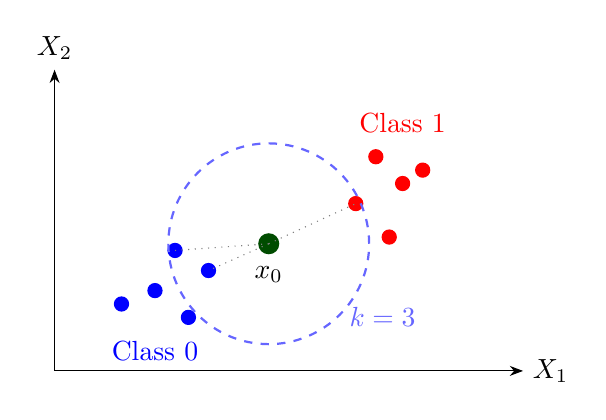
\begin{tikzpicture}[scale=0.85]
    
    % Axes
    \draw[->] (0,0) -- (7,0) node[right] {$X_1$};
    \draw[->] (0,0) -- (0,4.5) node[above] {$X_2$};
    
    % Class 0 points (blue squares)
    \foreach \x/\y in {1/1, 1.5/1.2, 2/0.8, 1.8/1.8, 2.3/1.5} {
        \filldraw[blue] (\x,\y) circle (3pt);
    }
    \node[blue] at (1.5, 0.3) {Class 0};
    
    % Class 1 points (red triangles)
    \foreach \x/\y in {4.5/2.5, 5/2, 5.5/3, 4.8/3.2, 5.2/2.8} {
        \filldraw[red] (\x,\y) circle (3pt);
    }
    \node[red] at (5.2, 3.7) {Class 1};
    
    % New point
    \filldraw[black!70!green, thick] (3.2,1.9) circle (4pt);
    \node[below] at (3.2,1.7) {$x_0$};
    
    % Neighborhood circle k=3
    \draw[dashed, thick, blue!60] (3.2,1.9) circle (1.5);
    \node[blue!60] at (4.9, 0.8) {$k=3$};
    
    % Lines to nearest neighbors
    \draw[dotted, gray] (3.2,1.9) -- (2.3,1.5);
    \draw[dotted, gray] (3.2,1.9) -- (1.8,1.8);
    \draw[dotted, gray] (3.2,1.9) -- (4.5,2.5);
    
    \end{tikzpicture}
    
    \vspace{0.3em}
    \textbf{Example with $k=3$:}
    \begin{itemize}
        \item 3 nearest neighbors: 2 from Class 0 (blue), 1 from Class 1 (red).
        \item Majority vote $\Rightarrow$ Predict Class 0. \quad $\hat{P}(\text{Class 0}) = 2/3$.
    \end{itemize}
\end{frame}


% Slide: KNN — Algorithm
\begin{frame}{KNN: Algorithmic Implementation}
    \small
    \begin{itemize}
    \item Given the local probability estimator defined previously,
    KNN operationalizes it through the following steps. For a query point $x_0$:
    \begin{enumerate}
        \item Choose the number of neighbors $k$.
        \item Compute distances $d(x_0, x_i)$ for all training observations.
        \item Identify the neighbor set $\mathcal{N}_k(x_0)$.
        \item Compute $\hat{p}_c(x_0)$ using neighbor frequencies.
        \item Assign class $\hat{Y}(x_0)$ by maximizing $\hat{p}_c(x_0)$.
    \end{enumerate}
    \item Remarks:
    \begin{itemize}
        \item No parameters are estimated during training.
        \item All computation occurs at prediction time (``lazy learning'').
        \item hyperparameters: $\color{red}{k}$ (number of neighbors), $\color{red}{d}$ (distance metric)
    \end{itemize}
    \end{itemize}
\end{frame}



% Slide: KNN Bias-Variance Trade-off
\begin{frame}{KNN: Choice of $k$ and bias-variance trade-off}
    \small
    The hyperparameter $k$ controls the bias-variance trade-off.
    
    \begin{itemize}
        \item Small $k$ (e.g., $k=1$):
        \begin{itemize}
            \item Highly flexible, jagged boundary. Low bias, high variance.
            \item Sensitive to noise and outliers. Risk of overfitting.
        \end{itemize}
        \item Large $k$ (e.g., $k=n$):
        \begin{itemize}
            \item Smoother, more stable boundary. High bias, low variance.
            \item Robust to noise. Risk of underfitting.
        \end{itemize}
        \item Selecting $k$ in Practice:
        \begin{itemize}
            \item Use cross-validation to find optimal $k$.
            \item Common starting point: $k = \sqrt{n}$. Odd $k$ avoids ties in binary classification.
        \end{itemize}
    \end{itemize}
\end{frame}

% Slide: KNN Choice of k Illustration
\begin{frame}{KNN: Effect of $k$ (Illustration)}
    \centering
    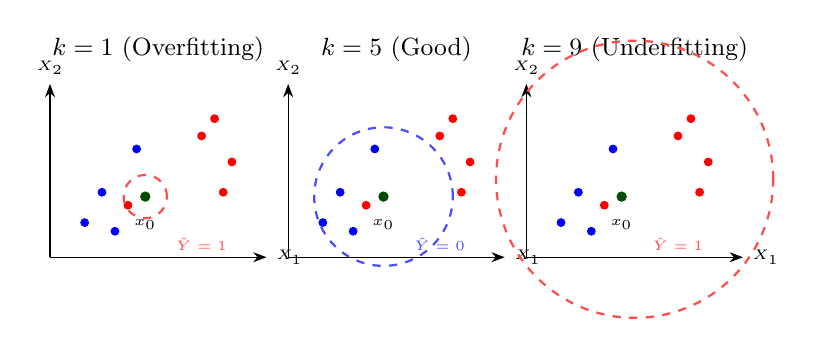
\begin{tikzpicture}[scale=0.55]
    
    % === Left panel: k=1 ===
    \node at (2.5, 4.8) {\small $k=1$ (Overfitting)};
    \draw[->] (0,0) -- (5,0) node[right] {\tiny $X_1$};
    \draw[->] (0,0) -- (0,4) node[above] {\tiny $X_2$};
    
    % Class 0 (blue)
    \foreach \x/\y in {0.8/0.8, 1.2/1.5, 1.5/0.6, 2/2.5} {
        \filldraw[blue] (\x,\y) circle (2.5pt);
    }
    % Class 1 (red)
    \foreach \x/\y in {3.5/2.8, 4/1.5, 3.8/3.2, 4.2/2.2} {
        \filldraw[red] (\x,\y) circle (2.5pt);
    }
    % Outlier (red in blue region)
    \filldraw[red] (1.8,1.2) circle (2.5pt);
    
    % Query point
    \filldraw[black!70!green] (2.2,1.4) circle (3pt);
    \node[below] at (2.2,1.1) {\tiny $x_0$};
    
    % Small circle for k=1
    \draw[dashed, thick, red!70] (2.2,1.4) circle (0.5);
    \node[red!70] at (3.5,0.3) {\tiny $\hat{Y}=1$};
    
    % === Middle panel: k=5 ===
    \begin{scope}[xshift=5.5cm]
    \node at (2.5, 4.8) {\small $k=5$ (Good)};
    \draw[->] (0,0) -- (5,0) node[right] {\tiny $X_1$};
    \draw[->] (0,0) -- (0,4) node[above] {\tiny $X_2$};
    
    % Class 0 (blue)
    \foreach \x/\y in {0.8/0.8, 1.2/1.5, 1.5/0.6, 2/2.5} {
        \filldraw[blue] (\x,\y) circle (2.5pt);
    }
    % Class 1 (red)
    \foreach \x/\y in {3.5/2.8, 4/1.5, 3.8/3.2, 4.2/2.2} {
        \filldraw[red] (\x,\y) circle (2.5pt);
    }
    % Outlier (red in blue region)
    \filldraw[red] (1.8,1.2) circle (2.5pt);
    
    % Query point
    \filldraw[black!70!green] (2.2,1.4) circle (3pt);
    \node[below] at (2.2,1.1) {\tiny $x_0$};
    
    % Medium circle for k=5
    \draw[dashed, thick, blue!70] (2.2,1.4) circle (1.6);
    \node[blue!70] at (3.5,0.3) {\tiny $\hat{Y}=0$};
    \end{scope}
    
    % === Right panel: k=9 (all) ===
    \begin{scope}[xshift=11cm]
    \node at (2.5, 4.8) {\small $k=9$ (Underfitting)};
    \draw[->] (0,0) -- (5,0) node[right] {\tiny $X_1$};
    \draw[->] (0,0) -- (0,4) node[above] {\tiny $X_2$};
    
    % Class 0 (blue)
    \foreach \x/\y in {0.8/0.8, 1.2/1.5, 1.5/0.6, 2/2.5} {
        \filldraw[blue] (\x,\y) circle (2.5pt);
    }
    % Class 1 (red)
    \foreach \x/\y in {3.5/2.8, 4/1.5, 3.8/3.2, 4.2/2.2} {
        \filldraw[red] (\x,\y) circle (2.5pt);
    }
    % Outlier (red in blue region)
    \filldraw[red] (1.8,1.2) circle (2.5pt);
    
    % Query point
    \filldraw[black!70!green] (2.2,1.4) circle (3pt);
    \node[below] at (2.2,1.1) {\tiny $x_0$};
    
    % Large circle covering all points
    \draw[dashed, thick, red!70] (2.5,1.8) circle (3.2);
    \node[red!70] at (3.5,0.3) {\tiny $\hat{Y}=1$};
    \end{scope}
    
    \end{tikzpicture}
    
    \vspace{0.3em}
    \small
    \begin{itemize}
        \item $k=1$: Only the red outlier $\Rightarrow$ misclassification.
        \item $k=5$: 4 blue, 1 red $\Rightarrow$ correct (Class 0).
        \item $k=9$: 4 blue, 5 red $\Rightarrow$ predicts global majority, ignores local structure.
    \end{itemize}
\end{frame}




% Slide: KNN — Distance Metrics and Feature Scaling
\begin{frame}{KNN: Choice of $d$ and curse of dimensionality}
    \small
    \begin{itemize}
    \item The definition of ``nearest'' depends on the distance metric $d(x, x')$.
    
    \item Common choices:
    \begin{itemize}
        \item Euclidean (L2): $d(x, x') = \sqrt{\sum_{j=1}^{p} (x_j - x'_j)^2}$ \quad (most common)
        \item Manhattan (L1): $d(x, x') = \sum_{j=1}^{p} |x_j - x'_j|$ \quad (robust to outliers)
        \item Cosine: $d(x, x') = 1 - \frac{x \cdot x'}{\|x\| \|x'\|}$ \quad (text/high-dim sparse data)
    \end{itemize}
    \item Critical preprocessing — Feature Scaling:
    \begin{itemize}
        \item Features with larger scales dominate the distance calculation.
        \item Standardization is essential: $\tilde{x}_j = \frac{x_j - \mu_j}{\sigma_j}$.
    \end{itemize}
    \end{itemize}
\end{frame}


% Slide: KNN — Dimensionality and Computation
\begin{frame}{KNN: Dimensionality and Computation}
    \small
    \begin{itemize}
        \item Curse of Dimensionality:
        \begin{itemize}
            \item As the dimension $p$ increases, observations become sparse in the feature space.
            \item ``Local'' neighborhoods may no longer be meaningfully local.
            \item To see this, note that to capture a fraction $r$ of the data in $p$ dimensions, a hypercube must have edge length $r^{1/p}$. Consider the example $r=0.1$:
            \begin{itemize}
                \item $p=2 \Rightarrow 0.32$
                \item $p=10 \Rightarrow 0.80$
                \item $p=100 \Rightarrow 0.98$
            \end{itemize}
        \end{itemize}
        
        \vspace{0.3em}
        \item Computational Implications:
        \begin{itemize}
            \item Training cost is negligible (data storage only).
            \item Prediction requires distance computation to all $n$ observations:
            $O(np)$ per query.
        \end{itemize}
    
        \item Practical Responses:
        \begin{itemize}
            \item Dimensionality reduction (feature selection, PCA).
            \item Distance metrics adapted to high-dimensional data (e.g.\ cosine similarity).
            \item Approximate nearest-neighbor methods for large datasets.
        \end{itemize}
    \end{itemize}
\end{frame}

% Slide: Curse of Dimensionality Illustration
\begin{frame}{KNN: Curse of Dimensionality (Illustration)}
    \centering
    To capture fraction $r$ of data, neighborhood edge length $= r^{1/p}$.
    
    \vspace{0.5em}
    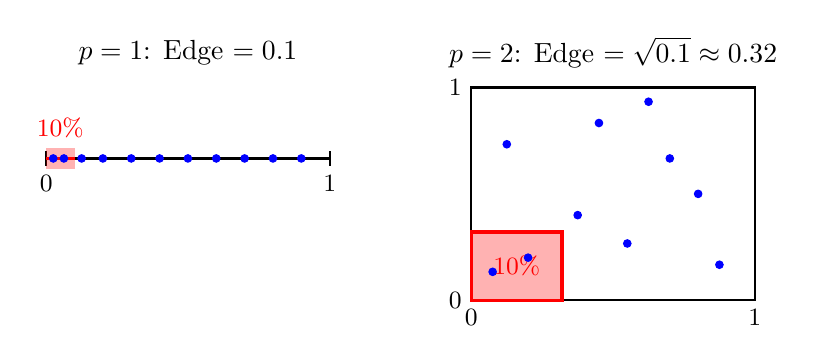
\begin{tikzpicture}[scale=0.9]
    
    % === Left panel: p=1 ===
    \node at (2, 3.5) {$p=1$: Edge $= 0.1$};
    
    % 1D line from 0 to 1
    \draw[thick] (0,2) -- (4,2);
    \draw[thick] (0,1.9) -- (0,2.1);
    \node[below] at (0,1.9) {\small $0$};
    \draw[thick] (4,1.9) -- (4,2.1);
    \node[below] at (4,1.9) {\small $1$};
    
    % Highlight 10% interval
    \draw[very thick, red] (0,2) -- (0.4,2);
    \fill[red, opacity=0.3] (0,1.85) rectangle (0.4,2.15);
    \node[red, above] at (0.2,2.15) {\small $10\%$};
    
    % Scattered points
    \foreach \x in {0.1, 0.25, 0.5, 0.8, 1.2, 1.6, 2.0, 2.4, 2.8, 3.2, 3.6} {
        \filldraw[blue] (\x,2) circle (1.5pt);
    }
    
    % === Right panel: p=2 ===
    \begin{scope}[xshift=6cm]
    \node at (2, 3.5) {$p=2$: Edge $= \sqrt{0.1} \approx 0.32$};
    
    % 2D box from 0 to 1
    \draw[thick] (0,0) rectangle (4,3);
    \node[below] at (0,0) {\small $0$};
    \node[below] at (4,0) {\small $1$};
    \node[left] at (0,0) {\small $0$};
    \node[left] at (0,3) {\small $1$};
    
    % Highlight 10% square (edge = 0.32 * 4 = 1.28 in scaled units)
    \fill[red, opacity=0.3] (0,0) rectangle (1.28,0.96);
    \draw[very thick, red] (0,0) rectangle (1.28,0.96);
    \node[red] at (0.64,0.48) {\small $10\%$};
    
    % Scattered points
    \foreach \x/\y in {0.3/0.4, 0.8/0.6, 1.5/1.2, 2.2/0.8, 2.8/2.0, 3.2/1.5, 0.5/2.2, 1.8/2.5, 3.5/0.5, 2.5/2.8} {
        \filldraw[blue] (\x,\y) circle (1.5pt);
    }
    \end{scope}
    
    \end{tikzpicture}
    
    \vspace{0.5em}
    \small
    \begin{itemize}
        \item In 1D, capturing 10\% of data requires only 10\% of the range.
        \item In 2D, capturing 10\% of data requires 32\% of each axis.
        \item As $p \to \infty$, ``local'' neighborhoods span nearly the entire space.
    \end{itemize}
\end{frame}







\section{Unsupervised Learning}

% Slide 1: Overview
\begin{frame}{Unsupervised Learning: Overview}
    \small
    \begin{itemize}
        \item Setup: We observe input vectors $X_1, \dots, X_n$, but no response $Y$.
        \[
            \D = \{x_1, x_2, \dots, x_n\}.
        \]
        \item Challenge: Without an observed target, there is no explicit loss function to guide learning.
        \item Goal: Using only the joint distribution of $X$, we aim to:
        \begin{itemize}
            \item Identify latent groupings or patterns among observations.
            \item Construct low-dimensional representations preserving essential structure.
            \item Characterize salient features of $P(X)$.
        \end{itemize}
    \end{itemize}
\end{frame}


% Slide 2: Clustering Definitions
\begin{frame}{Task 1: Clustering (Definitions)}
    \small
    \begin{itemize}
        \item Setup:
        We observe data $\{x_i\}_{i=1}^n$ drawn from a single, unknown distribution $P(X)$.
        
        \item Definition:
        Clustering partitions observations into groups using only information in $X$,
        without observing class labels or outcomes.
        
        \item Objective:
        Construct a partition $\{C_1,\dots,C_K\}$ such that:
        \begin{itemize}
            \item Observations within a cluster are similar according to a chosen metric.
            \item Observations across clusters are dissimilar.
        \end{itemize}
        
        \item Interpretation:
        \begin{itemize}
            \item Clusters provide a discrete summary of structure in $P(X)$
            (e.g.\ regions of high density or distinct geometric patterns).
            \item In some models, clusters may be interpreted as latent components of a mixture distribution.
        \end{itemize}
    \end{itemize}
\end{frame}

\begin{frame}{Task 1: Clustering (Example \& Mechanism)}
    \small
    \begin{itemize}
        \item Example:
        \textit{Market Segmentation}.  
        Given customer spending histories $X$, group customers with similar behavior.
        
        \item Mechanism: K-Means Clustering. Approximate the data distribution by $K$ representative centers and solve
        \[
            \min_{C_1,\dots,C_K}
            \sum_{k=1}^K \sum_{i \in C_k} \|x_i - \mu_k\|^2,
        \]
        where $\mu_k$ is the centroid of cluster $k$.
        
        \item Algorithm (Lloyd’s Algorithm):
        \begin{itemize}
            \item Initialize centroids $\{\mu_k^{(0)}\}_{k=1}^K$.
            
            \item Assignment:
            \[
                i \in C_k^{(t)}
                \iff
                \|x_i - \mu_k^{(t)}\|
                \le
                \|x_i - \mu_j^{(t)}\| \;\; \forall j.
            \]
            
            \item Update:
            \[
                \mu_k^{(t+1)}
                =
                \frac{1}{|C_k^{(t)}|}
                \sum_{i \in C_k^{(t)}} x_i.
            \]
            
            \item Iterate until assignments stabilize.
        \end{itemize}
    \end{itemize}
\end{frame}



% Slide: Task 2 — Dimensionality Reduction (Definitions)
\begin{frame}{Task 2: Dimensionality Reduction (Definitions)}
    \small
    \begin{itemize}
        \item Setup:
        Observations $\{x_i\}_{i=1}^n$ lie in a high-dimensional space $\mathbb{R}^p$.
        
        \item Definition:
        Dimensionality reduction constructs a low-dimensional representation of $X$
        using only information in $X$.
        
        \item Objective:
        Find a mapping
        \[
            x_i \in \mathbb{R}^p \;\longmapsto\; z_i \in \mathbb{R}^q, \quad q \ll p,
        \]
        such that essential structure in the data is preserved.
        
        \item Interpretation:
        \begin{itemize}
            \item The low-dimensional representation captures dominant patterns in $P(X)$.
            \item Reduces noise and redundancy while retaining informative variation.
        \end{itemize}
    \end{itemize}
\end{frame}


% Slide: Task 2 — Dimensionality Reduction (Example & Mechanism)
\begin{frame}{Task 2: Dimensionality Reduction (Example \& Mechanism)}
    \small
    \begin{itemize}
        \item Example:
        \textit{Visualizing Genetic Data}.  
        Gene expression levels for $p=10{,}000$ genes observed across $n=50$ patients;
        direct visualization in $\mathbb{R}^p$ is infeasible.
        
        \item Mechanism: Principal Component Analysis (PCA)
        
        PCA seeks low-dimensional projections of the form
        $Z_j = \phi_j^\top X$, where directions $\{\phi_j\}$ are chosen sequentially.
        
        \item First Principal Component:
        \begin{itemize}
            \item Choose $\phi_1$ to maximize variance:
            \[
                \phi_1
                =
                \arg\max_{\|\phi\|=1}
                \text{Var}(\phi^\top X).
            \]
        \end{itemize}
        
        \item Subsequent Components:
        \begin{itemize}
            \item For $j \ge 2$, choose
            \[
                \phi_j
                =
                \arg\max_{\|\phi\|=1}
                \text{Var}(\phi^\top X)
                \quad
                \text{s.t. } \phi^\top \phi_\ell = 0 \;\; \forall \ell < j.
            \]
            \item This enforces orthogonality and ensures components are uncorrelated.
        \end{itemize}
        
    \end{itemize}
\end{frame}


% Slide: Task 3 — Density Estimation (Definitions)
\begin{frame}{Task 3: Density Estimation (Definitions)}
    \small
    \begin{itemize}
        \item Setup:
        Observations $\{x_i\}_{i=1}^n$ are drawn from an unknown distribution $P(X)$.
        
        \item Definition:
        Density estimation aims to estimate the probability distribution $P(X)$ itself.
        
        \item Objective:
        Construct an estimator $\hat{p}(x)$ of the data density $p(x)$
        using only the observed sample.
        
        \item Interpretation:
        \begin{itemize}
            \item Provides a global, probabilistic description of $P(X)$.
            \item Serves as a foundation for anomaly detection, simulation, and likelihood-based analysis.
        \end{itemize}
    \end{itemize}
\end{frame}

% Slide: Task 3 — Density Estimation (Example & Mechanism)
\begin{frame}{Task 3: Density Estimation (Example \& Mechanism)}
    \small
    \begin{itemize}
        \item Example:
        Estimate the distribution of income, asset returns, or firm productivity
        using only observed data $\{x_i\}_{i=1}^n$.
        
        \item Mechanism: Kernel Density Estimation (KDE)
        
        KDE estimates the density at a point $x$ by locally averaging nearby observations:
        \[
            \hat{p}(x)
            =
            \frac{1}{nh}
            \sum_{i=1}^n
            K\!\left(\frac{x - x_i}{h}\right),
        \]
        where $K(\cdot)$ is a kernel function and $h>0$ is a bandwidth.
        
        \item Algorithmic Interpretation:
        \begin{itemize}
            \item Center a kernel $K$ at each observation $x_i$.
            \item Evaluate proximity using the scaled distance $(x-x_i)/h$.
            \item Average the contributions across all observations.
        \end{itemize}
        
        \item Bandwidth Choice:
        \begin{itemize}
            \item Small $h$: highly local averaging (low bias, high variance).
            \item Large $h$: strong smoothing (high bias, low variance).
        \end{itemize}
    \end{itemize}
\end{frame}

\begin{frame}{References}
    \begin{thebibliography}{10}
        
        \bibitem{hastie}
        James, G., Witten, D., Hastie, T., Tibshirani, R. (2021).
        \newblock \textit{An Introduction to Statistical Learning with Applications in Python}.
        \newblock Springer.
        \newblock \url{https://www.statlearning.com/}
        

        
    \end{thebibliography}
\end{frame}

\end{document}